\documentclass[11pt, twoside]{article}

\usepackage[parfill]{parskip}
\usepackage{amsmath}
\usepackage{gensymb}
\usepackage{geometry} 
\usepackage{graphicx, caption}
\usepackage{listings}
\usepackage{natbib}
\usepackage{placeins}
\usepackage{rotating}
\usepackage{textgreek}

\lstset{
  basicstyle=\small\ttfamily,
  columns=flexible,
  breaklines=true
}

\geometry{
  a4paper,
  left=20mm,
  top=20mm,
}

\begin{document}

\title{Simulating the ZetaSDR radio}
\author{Jason Leake}
\date{April 2019}
\maketitle
\section{Introduction}
The ZetaSDR radio \citep{ly1gp:2007}, designed by a Lithuanian radio
amateur, call sign LY1GP, is a simple direct conversion radio receiver
with a very small part count and forms the front end for a software
defined radio. The output from it is an analogue inphase and
quadrature signal, that allows the baseband to be extracted from
several different forms of modulation, for example frequency
modulation and quadrature amplitude modulation.

This program is simulates the operation of the Tayloe mixer that forms
the core of the ZetaSDR -- the 74HC4052 \citep{Motorola:1996}, and the
Johnson counter that drives it, producing the response to a simulated
amplitude modulated RF signal.  I wrote the program to see what ideal
time domain waveforms should look like on an oscilloscope as an
informal aid to constructing and optimising the radio.

Whilst this document contains a back-of-an-envelope analysis of the
operation of the mixer, the reader is referred to \cite{Soer:2007} for
a far more thorough examination.

The source code for the simulation is {\texttt program.cpp}, and
{\texttt plot.py} generates the plots from its CSV format output
files.  The program works on instantaneous samples of a simulated
incoming signal using the transformations that key components apply to
it, rather than employing a circuit solver.

The program was written for Ubuntu Linux is dependent upon several
packages, which can be installed via:

\begin{lstlisting}
sudo apt-get install make g++ librtlfilter-dev python3 python3-matplotlib texlive-all
\end{lstlisting}

Generating this PDF document is achieved by:

\begin{lstlisting}
make zetasdr.pdf
\end{lstlisting}

\begin{sidewaysfigure}
  \center
  \captionsetup{width=.8\linewidth}
  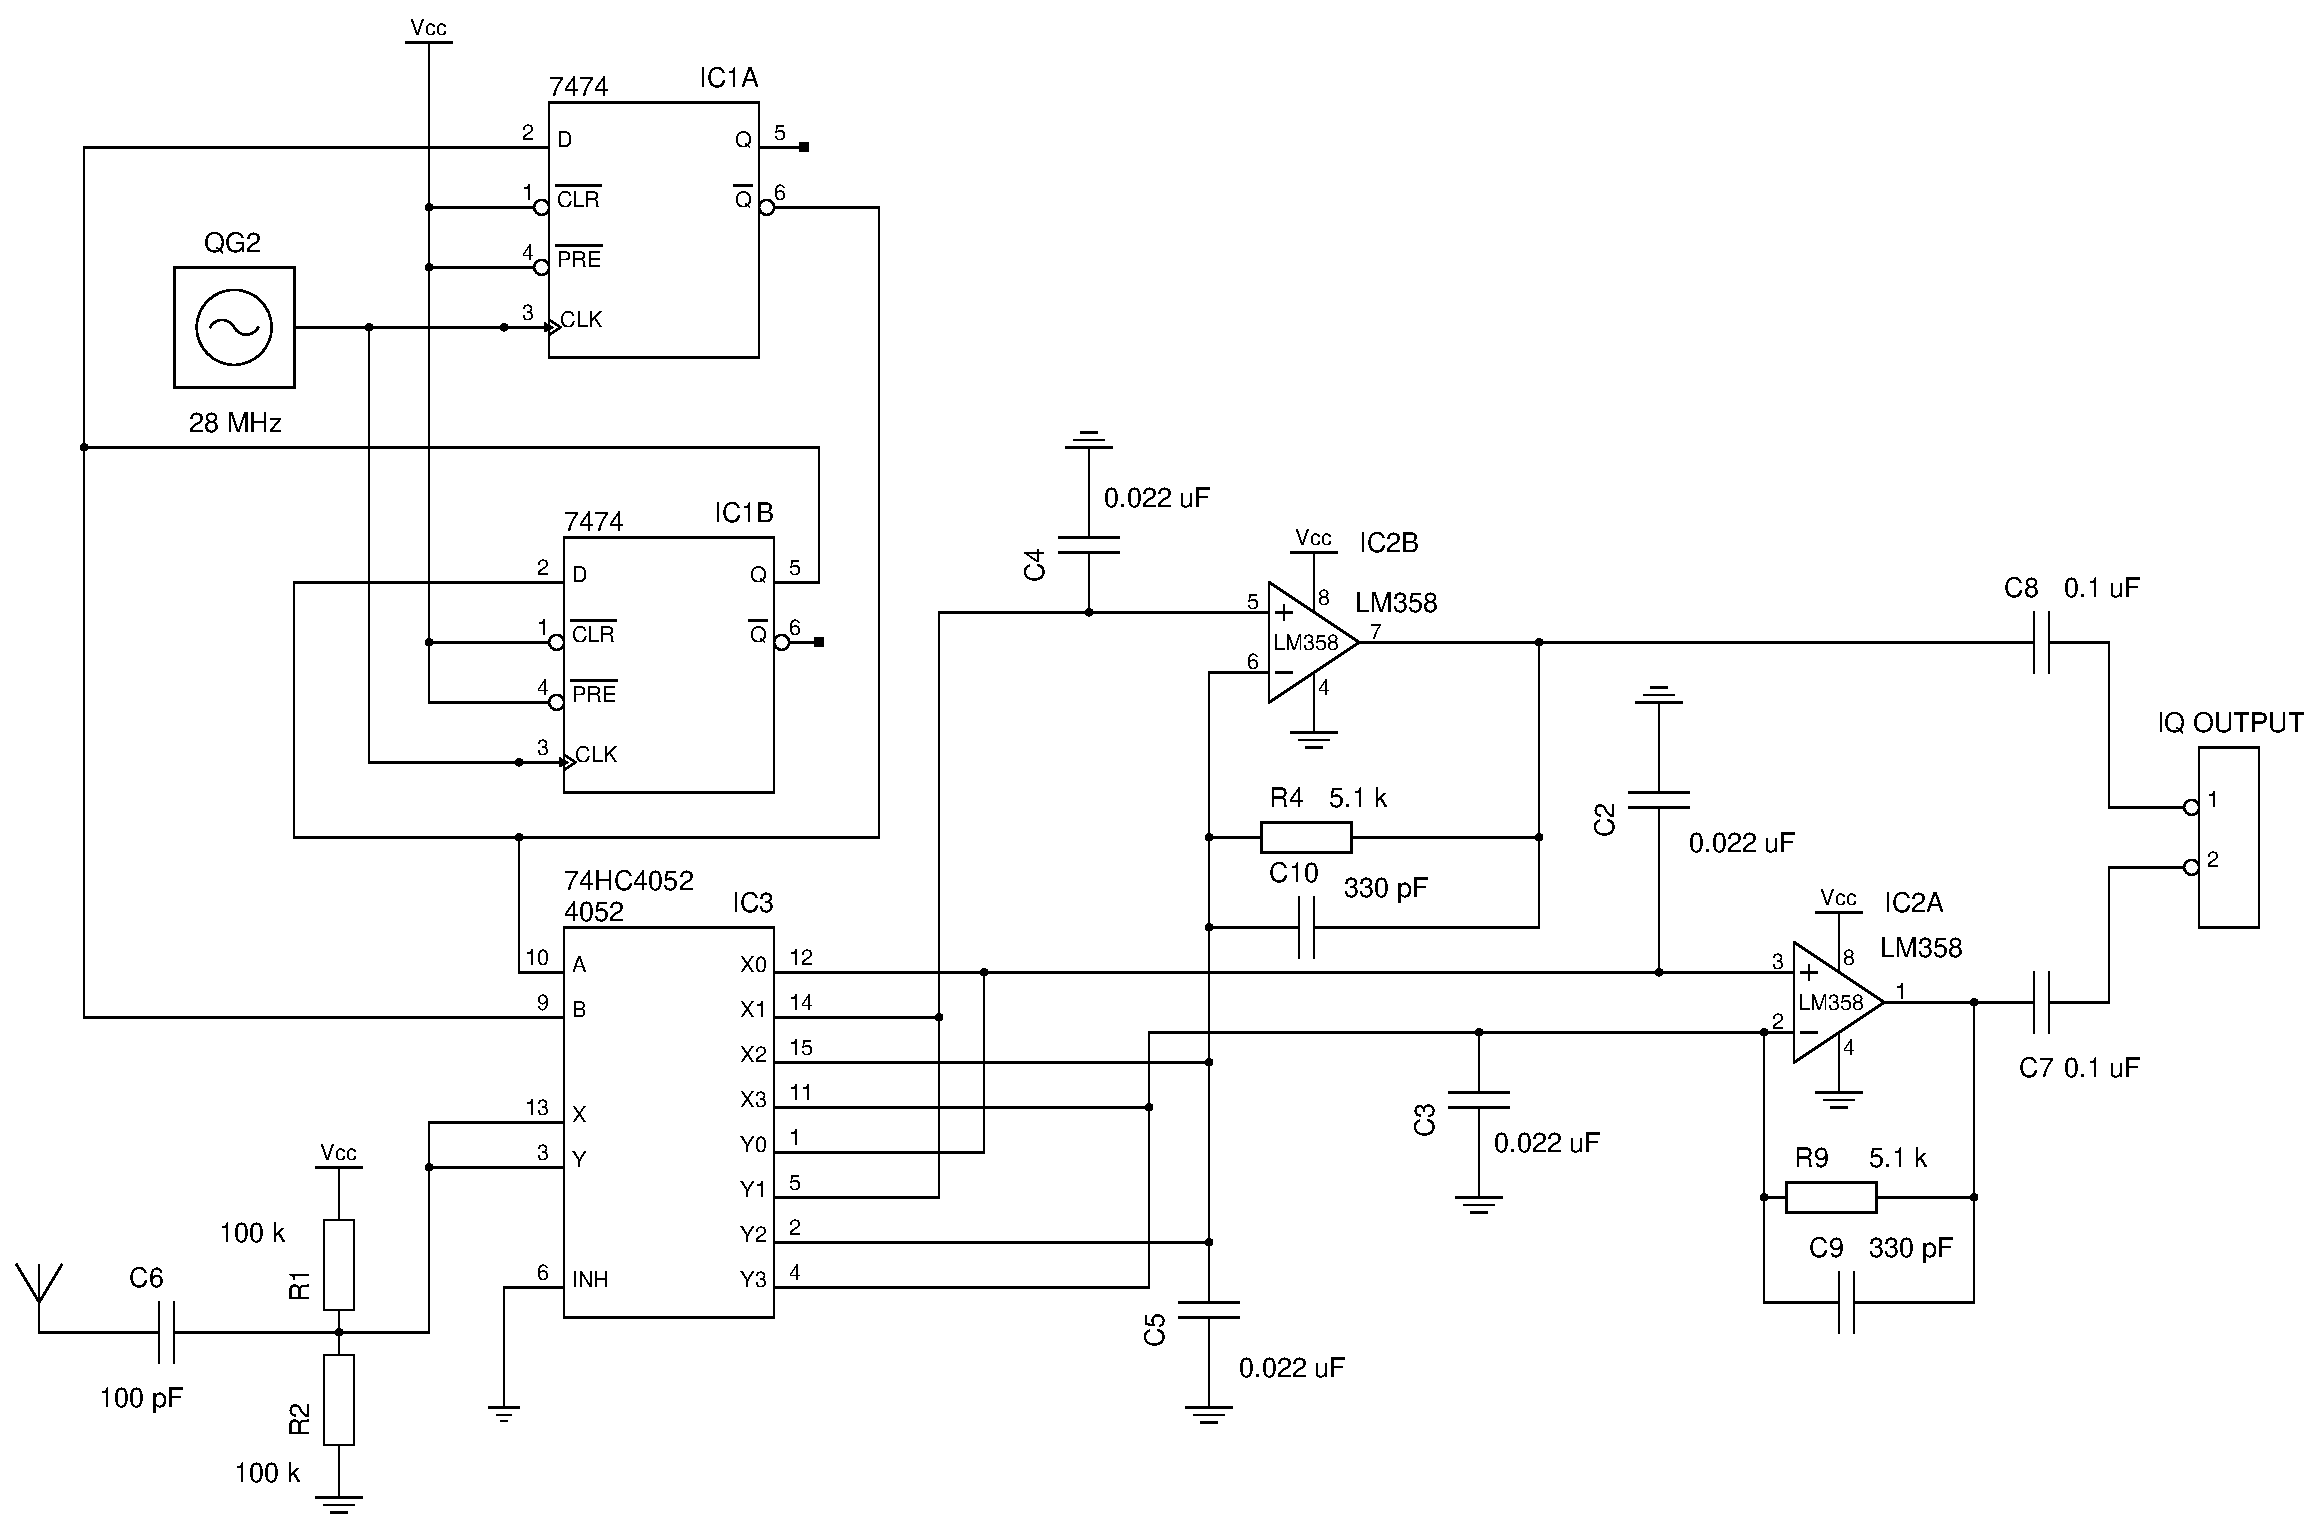
\includegraphics[width=.8\linewidth]{circuit.eps}
  \caption{ZetaSDR schematic (after \cite{ly1gp:2007})}
  \label{figure:schematic}
\end{sidewaysfigure}

\section{Operation of the ZetaSDR}

The incoming RF electromagnetic signal induces a small electrical
current in the antenna.  The current passes across capacitor C6
(Figure~\ref{figure:schematic}) which acts as a high pass filter,
blocking DC from passing from the receiver circuit to the antenna,
which could otherwise cause problems with preamplifiers.

A 2.5 volt bias is applied to the RF signal by the voltage divider
R1/R2 so that the signal oscillates around 2.5 volts instead of 0
volts.  This means that the rest of the circuit is dealing with a
signal in the middle of its normal operating range instead of around 0
volts where non-linearity in the response will be great even if it can
respond at all.

\subsection{Tayloe quadrature product detector}

The ZetaSDR uses a Tayloe quadrature product detector
\citep{Tayloe:2013, Tayloe:2001}, often informally called a Tayloe
mixer, to demodulate the signal.  This is a type of quadrature
sampling detector, a switching mixer that produces quadrature (IQ)
signals.  The ZetaSDR implementation uses a 74HC4052 analogue
multiplexer/demultiplexer and capacitors to implement an integrator.
It samples, averages and holds the RF signal on each quarter cycle,
sending the first and third quarter samples to the I output, and the
second and fourth quarter samples to the Q output.

The 74HC4052 is a twin channel analogue multiplexer/demultiplexer.
One channel has an input, X, and switches it to one of four outputs,
X0 $\rightarrow$ X3 depending on the state of the digital inputs A and
B (as shown in Table~\ref{table:74HC4052}).  If output X{\it n} is
enabled then the impedance between it and X is around 70 {\ohm}
(depending on supply voltage), and if not enabled then the path is
open circuit.  The device is bidirectional, but this is not relevant
here, for the purposes of the ZetaSDR it is enough that the input from
the antenna (X) is switched to one of the four outputs X1
$\rightarrow$ X4. The other 74HC4052 channel has an input called Y,
switching to Y1 $\rightarrow$ Y4.  The circuit uses both channels in
parallel to halve the impedance seen across the device from about 70
{\ohm} to 35 {\ohm}.

\begin{table}[ht]
  \center
  \begin{tabular}{|l| l| l| l|}
    \hline
    A & B & X & Y  \\
    \hline
    \hline
    0 &0& X0& Y0\\
    0 &1& X1& Y1\\
    1 &0& X2& Y2\\
    1 &1& X3& Y3\\
    \hline
  \end{tabular}
  \caption{Operation of 74HC4052}
  \label{table:74HC4052}
\end{table}

The inputs A and B are driven by a Johnson counter (also called a
twisted ring counter) made from two D-type flip flops.  This provides
two binary signals, connected to A and B, that change on every clock
cycle.  The clock is supplied by the QG2 local oscillator. The counter
operates as a 2 bit wide shift register, with the last bit value
being inverted and fed into the first bit of the shift register on
each clock cycle, so generating a repeating sequence 00, 01, 11, 10.
The local oscillator runs at four times the frequency of the RF
carrier, producing a new bit pattern in the Johnson counter, and thus
switching the 74HC4052, on every quarter cycle of the RF carrier.

Hence, each of the four pairs of outputs X0/Y0, X1/Y1, X2/Y2 and X3/Y3
receive a quarter cycle of the RF signal.  The outputs connect to the
sampling capacitors that charge/discharge as the RF carrier signal is
applied to them but hold their voltage when the corresponding 74HC4052
output is disabled and so in its high impedance state.

The amplitude of the RF carrier depends on the incoming signal
strength and the quality of the antenna and preamplifier, so I picked
an arbitrary value of 1 mV for the simulation program.

The waveform shapes produced by the simulation will be the same for
smaller voltages, albeit with a smaller amplitude since the simulation
does not model the noise in the system.

Since the local oscillator output is the Johnson counter clock, the
flip flops making up the counter change when the local oscillator
signal transitions from a voltage corresponding to logic 0 to logic 1.
The simulation sets the logic 1 transition to a conventional 2.4
volts, and since the local oscillator has a swing of 5 volts, the
clock occurs just below the midpoint on the local oscillator upswing.

Because the Johnson counter produces the sequence 00, 01, 11, 10, the
first and third quarters of the RF carrier cycle are selected using
outputs X0 and X3 respectively, and the second and fourth using X1 and
X2.

The voltage on the sampling capacitors C2 and C3 are shown in
Figure~\ref{figure:C2C3simple}. The local oscillator is set to have a
range of 0--5 volts, and have its 0{\degree} point at the 0{\degree},
90{\degree}, 180{\degree} and 270{\degree} positions of the RF
carrier.  In this idealised simulation the Johnson counter therefore
changes state very slightly before this point, when the local
oscillator voltage is rising through 2.4 volts.

In practice, it is unlikely that the local oscillator will be in phase
with the RF carrier, and there will be small delays in the Johnson
counter logic and the 74HC4052 operation.

The two sampling capacitors are also connected to the differential
inputs of an active low pass filter that both amplifies and filters
the difference between the two voltages.  In the simulation, the low
pass filters have an infinite input impedance. The final output
voltage is shown on the lower plot in Figure~\ref{figure:C2C3simple}
-- the effect of taking the difference between the two signals, which
will be normally be similar but of opposite polarity, is to produce a
signal of double the size of each.  The corresponding voltages on the
other pair of capacitors, C4 and C5, are shown in
Figure~\ref{figure:C4C5simple}.

In the \cite{LY1GP:2007} schematic, a 28.322 MHz local oscillator is
specified, but the simulation used a 28 MHz oscillator and hence a 7
MHz radio signal.


\begin{figure}
  \center
  \captionsetup{width=.8\linewidth}
  \includegraphics[width=.8\linewidth]{c2c3_unmodulated_voltage.png}
  \caption{Voltage on C2 and C3, ZetaSDR, when the local oscillator is
    in phase with the RF signal. The 74HC4052 switching leads the RF
    signal phase very slightly because its local oscillator derived
    clock changes logic state just below the midpoint on the local
    oscillator upswing.}
  \label{figure:C2C3simple}
\end{figure}


\begin{figure}
  \center
  \captionsetup{width=.8\linewidth}
  \includegraphics[width=.8\linewidth]{c4c5_unmodulated_voltage.png}
  \caption{Voltage on C4 and C5, ZetaSDR, when the local oscillator is
    in phase with the RF signal}
  \label{figure:C4C5simple}
\end{figure}

The sharp transitions and the short-lived spikes will be attenuated by
the active low pass filter stage.  Hence, the demodulator is producing
an output where the I signal is sampled at two points in the carrier
cycle 180{\degree} apart, and the Q signal is the signal sampled
90{\degree} on from those points in much the same way that the
multiplication by the respective local oscillator does it in a
conventional multiplying IQ mixer.

Hence, if the amplitude or phase of the signal does not change rapidly
during the sampling and we ignore the quarter cycles where the voltage
on the capacitors is changing, then for the I signal, the voltage at
capacitor C2 in Figure~\ref{figure:C2C3simple} is

\begin{equation*}
  s_1 = A cos(\theta) sin({\omega_b}t)
\end{equation*}

where:\\
\\
  ${\omega_b}$ is the baseband frequency in radians per second\\

$\theta$ is the phase difference between the carrier and the Johnson
counter transitions (and hence the 74HC4052 switching)

The voltage across C3 is:

\begin{align*}
  s_2 & = A cos(\theta) sin(\pi + {\omega_b}t) \\
  \\
  &= -A cos(\theta) sin({\omega_b}t)
\end{align*}

Because the active filter is the difference between the two voltages,
the filter output is:

\begin{equation}\label{eqn:tayloei}
  I = s_1 - s_2 = 2 A cos(\theta) sin({\omega_b}t)
\end{equation}

Hence, the difference into the active low pass filter, ignoring the
high frequency portion which results when one of the capacitors is
tracking the output from the 74HC4052 rather than holding its voltage,
is $2A sin(\theta) sin({\omega_b}t)$.

By the same reasoning, the Q signal formed from the voltage difference
between C4 and C5 is:

\begin{equation}\label{eqn:tayloeq}
  Q = 2 A sin(\theta) sin({\omega_b}t)
\end{equation}

\begin{figure}
  \center
  \captionsetup{width=.8\linewidth}
  \includegraphics[width=.8\linewidth]{c2c3_modulated_voltage.png}
  \caption{Voltage on C2 and C3 in the ZetaSDR, when the local
    oscillator is in phase with the RF carrier, and the 7 MHz carrier
    is amplitude modulated at 100 kHz}
  \label{figure:C2C3mod}
\end{figure}

\begin{figure}
  \center
  \captionsetup{width=.8\linewidth}
  \includegraphics[width=.8\linewidth]{c4c5_modulated_voltage.png}
  \caption{Voltage on C4 and C5, when the local oscillator is in phase
    with the RF carrier, and the 7 MHz carrier is amplitude modulated
    at 100 kHz}
  \label{figure:C4C5mod}
\end{figure}


The corresponding plots for a modulated signal are shown in
Figures~\ref{figure:C2C3mod} and \ref{figure:C4C5mod}. Many more RF
cycles are shown in these plots, and the 7 MHz carrier is amplitude
modulated at 100 kHz.  Although this is above the audio range, it
allows several AM cycles can be accommodated

\begin{figure}
  \center
  \captionsetup{width=.8\linewidth}
  \includegraphics[width=.8\linewidth]{c2c3_unmodulated_voltage_35.png}
  \caption{Voltage on C2 and C3 in the ZetaSDR, when the local
    oscillator leads the RF carrier by 35{\degree}}
  \label{figure:C2C3phase}
\end{figure}

\begin{figure}
  \center
  \captionsetup{width=.8\linewidth}
  \includegraphics[width=.8\linewidth]{c4c5_unmodulated_voltage_35.png}
  \caption{Voltage on C4 and C5 in the ZetaSDR, when the local
    oscillator leads the RF carrier by 35{\degree}}
  \label{figure:C4C5phase}
\end{figure}

In practice, the 74HC4052 switching will usually be more out of phase
with the RF carrier signal, and so something such as
Figure~\ref{figure:C2C3phase} (and Figure~\ref{figure:C4C5phase} for
the other pair of capacitors) is more likely.  The modulated versions
of these plot, over a larger number of carrier cycles, are shown in
Figures~\ref{figure:C2C3modphase} and \ref{figure:C4C5modphase} are
obtained.

Figure~\ref{figure:zetasdr_low_pass_phase} shows the I and Q signals
through a low pass filter and then combining them to extract the
baseband.  Because of the unusually high modulation frequency and
signal strength used in the simulation, a 500 kHz $2^{nd}$ order zero
gain low pass Butterworth filter is used instead of the higher gain
and lower frequency cutoff active low pass filters in the ZetaSDR
radio.

\begin{figure}
  \center
  \captionsetup{width=.8\linewidth}
  \includegraphics[width=.8\linewidth]{zetasdr_modulated_35_va.png}
  \caption{Voltage on C2 and C3 in the ZetaSDR, when the local
    oscillator leads the carrier by 35{\degree}, and the 7 MHz carrier
    is amplitude modulated at 100 kHz}
  \label{figure:C2C3modphase}
\end{figure}

\begin{figure}
  \center
  \captionsetup{width=.8\linewidth}
  \includegraphics[width=.8\linewidth]{zetasdr_modulated_35_vb.png}
  \caption{Voltage on C4 and C5 in the ZetaSDR, when the local
    oscillator leads the carrier by 35{\degree}, and the 7 MHz carrier
    is amplitude modulated at 100 kHz}
  \label{figure:C4C5modphase}
\end{figure}


\begin{figure}
  \center
  \captionsetup{width=.8\linewidth}
  \includegraphics[width=.8\linewidth]{zetasdr_modulated_35_d.png}
  \caption{ZetaSDR response to a 100 kHz amplitude modulated signal,
    when the local oscillator is 35{\degree} ahead of the RF
    carrier. Because of the high input signal amplitude and the high
    modulation frequency, the active low pass filters have been
    replaced with a $2^{nd}$ order low pass filter, but with unity
    gain and a cutoff frequency of 500 kHz.}
  \label{figure:zetasdr_low_pass_phase}
\end{figure}

\section{Comparison with an ideal multiplying IQ mixer}

A sinusoidally amplitude modulated RF signal, with a 100\% modulation
depth, double-sideband and full-carrier, is described by:

\begin{equation}
S = A sin({\omega_b}t) sin({\omega_c}t)
\end{equation}

where:\\
\\
$A$ is the signal amplitude\\
$\omega_b$ is the baseband frequency\\
$\omega_c$ is the carrier frequency \\
  $t$ is time\\

In a conventional multiplying IQ mixer, the I signal is produced by
mixing with a local oscillator with a phase difference $\theta$:

\begin{align*}
I =& A sin({\omega_b}t)  sin({\omega}_ct)sin({\omega}_ct + \theta) \\
\\
&= A sin({\omega_b}t)  \frac{cos(\theta) - cos(2 {\omega}_ct - \theta)}{2}
\\
&= \frac{A sin({\omega_b}t) cos(\theta)}{2} - \frac{cos(2 {\omega_c}t - \theta)}{2}
\end{align*}

Because

\begin{equation*}
  sin(\alpha) sin(\beta) = \frac{sin(\alpha + \beta) - sin(\alpha - \beta)}{2}
\end{equation*}

The Q signal is produced by mixing the incoming RF signal with a
similar local oscillator signal that is 90{\degree} out of phase with
the I local oscillator:


\begin{align*}
  Q& = A sin({\omega_b}t) cos({\omega}_ct) sin({\omega}_ct + \theta) \\
  \\
  & = A sin({\omega_b}t) \frac{sin(2{\omega}_ct + \theta) + sin(\theta)}{2}\\
  \\
& = \frac{A sin({\omega_b}t)sin(2{\omega}_ct + \theta)}{2} + \frac{A sin({\omega_b}t)sin(\theta)}{2}\\
\end{align*}

Because

\begin{equation*}
  cos(\alpha)sin(\beta) = \frac{(sin(\alpha + \beta) - sin(\alpha - \beta)}{2} 
\end{equation*}

In both cases, a low pass filter will remove the sum portion of the
signal at frequency $2{\omega_c}$ leaving only the difference
frequency:

\begin{equation*}
  I = \frac{A sin({\omega_b}t)cos(\theta)}{2}
\end{equation*}

\begin{equation*}
  Q = \frac{A sin({\omega_b}t)sin(\theta)}{2}
\end{equation*}

These two equations are of the same form as
Equations~\ref{eqn:tayloei} and \ref{eqn:tayloeq}, the ones for the
Tayloe quadrature product detector, demonstrating that it operates as
an IQ mixer.

The results of the simulation of an ideal multiplying IQ mixer are
shown in
Figures~\ref{figure:iq_mod}--\ref{figure:iq_mod_low_pass_phase} for
comparison with the Tayloe detector simulation plots above.

Like the IQ mixer output, the Tayloe detector in the ZetaSDR produces
sum and difference frequencies. The high frequency portion of detector
output signal is at $2\omega_c$, since the rapidly varying portion
gets through two cycles for each cycle of the RF carrier, although in
this case there are additional harmonics.  The detector capacitors are
intended to form an RC low pass filter with the resistance through the
74HC4052 to remove the sum frequency component (the Tayloe mixer
minimises the use of resistors to reduce noise).  However, the ZetaSDR
has an additional active low pass filter, so this filter is redundant,
and for this reason the detector capacitors can be deleted.

The cutoff frequency of the RC circuit is about 85 kHz if the
aggregate resistance through the pair of 74HC4052 channels in parallel
is 35 {\ohm} and the impedance of the antenna is 50 {\ohm}.
\cite{Tayloe:2013} says that effective resistance for filter
calculations is quadrupled if the signal is only connected for a
quarter of the time, but my simulation works at a small time step
level, so still sees the ``instantaneous'' cutoff at 85 kHz when the
capacitor is connected to the signal, and the capacitor voltage frozen
when it is disconnected.

The modulation frequencies used by the simulation are 83 kHz and 100
kHz, as a not entirely ideal compromise between being strongly
affected by this RC filter and being a sufficiently high frequency to
allow the plots to show at least one modulation cycle.

Perhaps the greatest weakness of the design is that it relies upon the
mixer to emphasise the tuned frequency over adjacent ones.  Perhaps
this is not such a problem in practice if the antenna can be tuned.

But to investigate this further, Figures~\ref{figure:adjacent} and
\ref{figure:tuned_adjacent} show simulations for a pair of signals
close to each other and the ZetaSDR radio tuned to one or other
signals.  The signal parameters are shown in
Table~\ref{table:adjacent}.  The conclusion from these simulations is
that the adjacent signal introduces very considerable distortion on
the demodulated signal that the radio is tuned to, although
Figures~\ref{figure:iq_adjacent} and \ref{figure:iq_tuned_adjacent}
show that an ideal IQ mixer without any additional tuning capability
also produces similarly distorted results.

\begin{table}[ht]
  \center
  \begin{tabular}{| l| c| r |}
    \hline
    Signal & Carrier & Amplitude \\
    & frequency & modulation \\
    && frequency \\
    \hline
    \hline
    Signal 1 & 7 MHz & 100 kHz \\
    Signal 2 & 7.5 MHz & 83 kHz\\
    \hline
  \end{tabular}
  \caption{Signals used in examining adjacent signal response}
  \label{table:adjacent}
\end{table}

\begin{figure}
  \center \captionsetup{width=.8\linewidth}
  \includegraphics[width=.8\linewidth]{iq_modulated_0.png}
  \caption{I/Q outputs using an ideal multiplying IQ mixer, when the
    local oscillator is in phase with the RF carrier, and the 7 MHz
    carrier is amplitude modulated at 100 kHz}
  \label{figure:iq_mod}
\end{figure}

\begin{figure}
  \center
    \captionsetup{width=.8\linewidth}
  \includegraphics[width=.8\linewidth]{iq_modulated_35.png}
  \caption{I/Q outputs using an ideal multiplying IQ mixer when the
    local oscillator leads the carrier by 35{\degree}, and the 7 MHz
    carrier is amplitude modulated at 100 kHz}
  \label{figure:iq_modphase}
\end{figure}

\begin{sidewaysfigure}
  \center
    \captionsetup{width=.8\linewidth}
  \includegraphics[width=.8\linewidth]{iq_modulated_35_d.png}
  \caption{I/Q outputs using an ideal multiplying IQ mixer, when the
    local oscillator is 35{\degree} ahead of the RF carrier, and with
    the I/Q signals passed through a $2^{nd}$ order low pass filter
    with a cutoff of 400 kHz to remove the $2{\omega_c}$ signal.
    Compare this ideal case with
    Figure~\ref{figure:zetasdr_low_pass_phase}.}
  \label{figure:iq_mod_low_pass_phase}
\end{sidewaysfigure}

\begin{sidewaysfigure}
  \center
  \captionsetup{width=.8\linewidth}
  \includegraphics[width=.8\linewidth]{zetasdr_adjacent_35.png}
  \caption{I and Q outputs from the ZetaSDR with the local oscillator
    starting 35{\degree} ahead of the carrier.  The second order low
    pass filter has a cutoff of 400 kHz. The signals present described
    in Table~\ref{table:adjacent}, with the local oscillator tuned to
    Signal 1.}
  \label{figure:adjacent}
\end{sidewaysfigure}

\begin{sidewaysfigure}
  \center \captionsetup{width=.8\linewidth}
  \includegraphics[width=.8\linewidth]{zetasdr_tuned_adjacent_35.png}
  \caption{I and Q outputs from the ZetaSDR tuned to Signal 2 in
    Table~\ref{table:adjacent}, and starting starting 35{\degree}
    ahead of the carrier.}
  \label{figure:tuned_adjacent}
\end{sidewaysfigure}

\begin{sidewaysfigure}
  \center
  \captionsetup{width=.8\linewidth}
  \includegraphics[width=.8\linewidth]{iq_adjacent_35_d.png}
  \caption{I and Q outputs from an ideal multiplying IQ mixer with the
    local oscillator tuned to Signal 1 in Table~\ref{table:adjacent},
    and starting starting 35{\degree} ahead of the carrier.}
  \label{figure:iq_adjacent}
\end{sidewaysfigure}


\begin{sidewaysfigure}
  \center
  \captionsetup{width=.8\linewidth}
  \includegraphics[width=.8\linewidth]{iq_tuned_adjacent_35_d.png}
  \caption{I and Q outputs from an ideal multiplying IQ mixer.  local
    oscillator is tuned to Signal 2 in Table~\ref{table:adjacent}, and
    starting starting 35{\degree} ahead of the
    carrier.}
  \label{figure:iq_tuned_adjacent}
\end{sidewaysfigure}

\begin{thebibliography}{9}
\bibitem[LY1GP(2007)]{ly1gp:2007}
  LY1GP (2007), {\it ZetaSDR for 40m band}
  \\\texttt{http://www.qrz.lt/ly1gp/SDR/}

\bibitem[Motorola(1996)]{Motorola:1996}
  Motorola (1996),
  {\it Analog Multiplexers/Demultiplexers High–Performance Silicon–Gate CMOS},
  \texttt{http://www.om3bc.com/datasheets/74HC4051.PDF}

\bibitem[Soer(2007)]{Soer:2007}
  Soer M (2007), 
  {\it Analysis and comparison of switch-based frequency converters}, MSc. thesis, University of Twente,
\texttt{https://essay.utwente.nl/58276/1/scriptie\_Soer.pdf}

\bibitem[Tayloe(2001)]{Tayloe:2001}
  Tayloe, D (2001), {\it Product detector and method therefor -- United States Patent No 6230000}, United States Patent and Trademark Office,
  \\\texttt{https://patentimages.storage.googleapis.com/ed/ec/5f/c214501bb441f1/US6230000.pdf}

\bibitem[Tayloe(2013)]{Tayloe:2013} 
  Tayloe, D (2013), {\it Ultra Low Noise, High Performance, Zero IF Quadrature Product Detector and Preamplifier},
  \\\texttt{https://wparc.us/presentations/SDR-2-19-2013/Tayloe\_mixer\_x3a.pdf}

\end{thebibliography}

\end{document}

